% Edit the captions to say what YOU want the reader to see.

\begin{figure}[htbp]
  \centering
  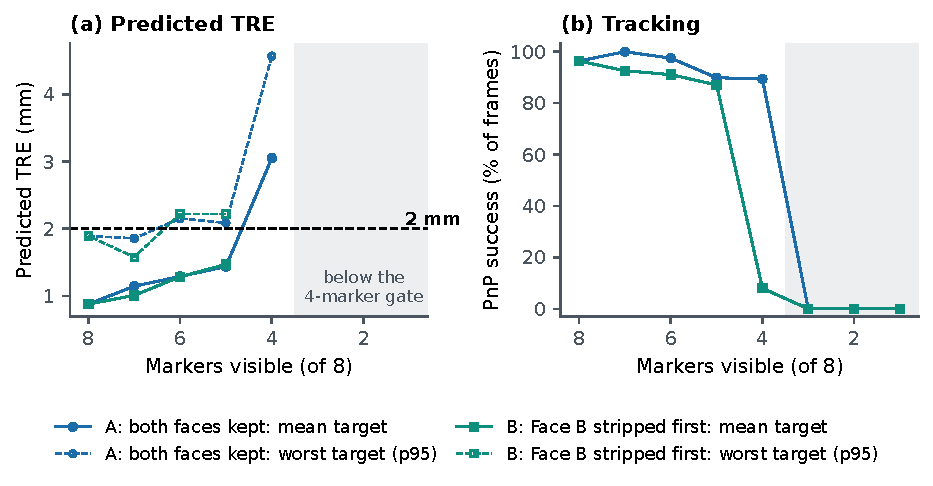
\includegraphics[width=\textwidth]{figures/fig_atp4_occlusion.pdf}
  \caption{ATP-4 occlusion. (a) Predicted TRE (mean over targets, and 95th percentile of the worst target) and (b) PnP success against the number of visible markers, covering markers progressively. In sequence A the last four markers are the near-junction cluster (IDs 0, 2, 5, 7); in sequence B they are all on Face A (TRE is not drawn where fewer than half the frames tracked). Both sequences share the 8-marker baseline recorded at the end of sequence A. Tracking is not attempted below four markers.}
  \label{fig:results:atp4}
\end{figure}

\begin{figure}[htbp]
  \centering
  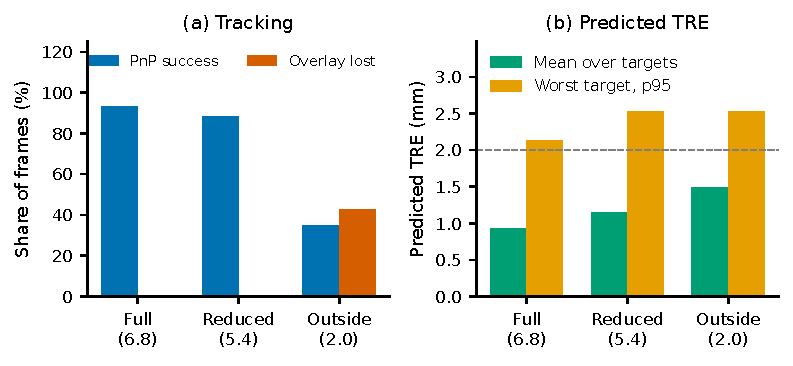
\includegraphics[width=\textwidth]{figures/fig_tier_comparison.pdf}
  \caption{Tracking and predicted TRE per envelope tier, pooled over the ATP-3 sweeps (frame-weighted). Mean detected markers per tier are in brackets under each label. Predicted TRE depends only on the visible marker set.}
  \label{fig:results:tiers}
\end{figure}
